\documentclass [a4paper,12pt,oneside,final]{report}
\addtolength{\skip\footins}{2pc plus 5pt}

\usepackage[top=2.5cm,bottom=2.5cm,right=2.5cm,left=2.5cm]{geometry}
\usepackage{natbib}
\usepackage[utf8]{inputenc}
\usepackage{multicol}
\usepackage{url}
\usepackage{subfiles}
\usepackage{nameref}
\usepackage{fontenc}
\usepackage{diagbox}

\usepackage{graphicx}
\usepackage{subcaption}
\usepackage{caption}

\usepackage{amssymb}
\usepackage{amsmath}
\usepackage{tabularx}

\usepackage{hyperref}

\usepackage[final]{pdfpages}
\usepackage{caption}
\graphicspath{ {figures/}}

\usepackage[ruled,vlined, onelanguage, linesnumbered]{algorithm2e}
\usepackage{glossaries}
\subfile{acronyms.tex}
\subfile{vocable}

\title{Rapport de stage}
\date{May 2022}

% \makeglossaries
\makenoidxglossaries

\begin{document}

\includepdf[pages=-]{page_de_garde.pdf}
\pagenumbering{roman}
\chapter*{Acknowledgement}
\addcontentsline{toc}{chapter}{Acknowledgement and Dedication}
\thispagestyle{empty}


\vspace{0.75cm}
\textit{This thesis was made possible thanks to the help of several people to whom I would like to express my gratitude.}
\vspace{0.75cm}

\textit{ First of all, I would like to thank my two supervisors in this work, Mr. Pedro Fillastre and Mr. Jean-Marc Brun. They were there when I needed answers, suggestions, advice and reviews that helped me to improve the quality of my work. I am grateful to them for their constant presence, their constructive criticism and their considerable efforts.}

\vspace{0.75cm}

\textit{I would also like to thank my supervisor Mr. Mohamed Nadif and the person in charge of training, for his immense help, as well as for all the advice and information he gave us with a degree of patience and professionalism throughout my course at the university.}
\vspace{0.75cm}


\textit{I would also like to express my sincere thanks to Mr. Sebastiao Correia, the manager of the Lab team at Talend, for offering me the opportunity to join the team, for his support, his guidance, his availability and his constant presence during this internship period.}
\vspace{0.75cm}


\textit{I would also like to thank everyone at Suresnes offices who welcomed me and made my integration easier, and especially the members of the Lab team for their opinions and constructive criticism.}
\vspace{0.75cm}


\textit{I would also like to thank the members of the jury who took the time to review and evaluate my work in the best possible way.}


\chapter*{Abstract}
\addcontentsline{toc}{chapter}{Abstract}

The continuous growth of the data in the hands of the companies has always
presented a real management problem, a problem that has been tackled by Talend
by developing and delivering its product
\href{https://www.talend.com/products/data-inventory/}{Data Inventory} offering
a set of functionalities to its clients. In order to increase the capabilities
of this tool, the Talend Lab team proposes to work on a research project aiming
to extract metadata from the data allowing it to easily detect similarities
between datasets. 

It is in this context that the present project takes place, where we explore the
literature related to dataset similarity detection and implement techniques to
efficiently extract metadata from any new dataset. We built during this project
a proof of concept that provides the user with the possibility to introduce and
index a new dataset, and to compute efficiently for a selected dataset, the
degree of similarity with the other dataset in the system. We scaled the
similarity detection from the level of datasets to the level of their columns
and we used the latter to deduce a score for the first.

This type of functionality can be used in different ways, we can use it to
suggest to the user to compare and merge two similar datasets, or to update the
records of one of them. We can also use it to detect the topic of the dataset if
the ones similar to it have already been tagged with their respective topics.

To build our solution, we tackle this topic as \acrfull{nns} problem, and we use
a method from the \acrfull{lsh} family which is Cross-Polytope LSH and we
combine it with Multi-Probe LSH to improve its indexation quality. This solution
has been tested on a benchmark that has been used in an internal project at
Talend, and it shows up that our solution achieves an accuracy of 60\% when it
comes to reproducing human-labelled similarities.

\vspace{2cm}
\textbf{Keywords:}
\acrlong{nns}, \acrlong{lsh}, Cross-Polytope, Data Fingerprinting, Indexation,
Similarity \& Dissimilarity Metrics
\tableofcontents
\clearpage
\listoffigures
\clearpage
\listofalgorithms
\clearpage

\pagenumbering{arabic}
\chapter*{Introduction}
\addcontentsline{toc}{chapter}{Introduction}

As data continues to grow, it is becoming increasingly critical for
organizations to be able to easily manage and sort their datasets, whether they
come from databases, files or other sources. For this purpose, Talend already
offers \href{https://www.talend.com/products/data-inventory/}{Talend Data
Inventory}, a tool that makes it easy to find and understand your data with
powerful and versatile search, provenance and dataset overview. It also helps to
identify data silos in all data sources and eliminates them with reusable and
shareable data assets.

In order to continuously improve the Talend Data Inventory quality of service,
Talend Lab team is interested in integrating a tool that can detect the
similarities between datasets, a functionality that can be used in different use
cases, the most relevant one is at the moment when the user introduces a new
dataset, we want to find the ones that are similar to it, and by providing this
information to the user we can propose some actions he can do, he can for
example compare and merge the similar datasets or update the existing one with
new records. Another use case is to assign a tag to a dataset according to the
tags of the ones that are similar to it, for example if we find that a dataset
is similar to two dataset with the tag "\textit{finance}", we can suggest this
same tag to the user.

In this work, we tackle the problem of detecting similarities between dataset as
a \Acrfull{nns} problem, we explore the state of the art with focusing on
\Acrfull{lsh} methods and we study their different versions and the metric they
consider.

We present in the second place the solution built during this internship, in
which we use a method of the \acrshort{lsh} family called Cross-Polytope, our
goal is to scale its idea that was initiated to work at row level and get it
work at the column level, we propose for this a set of preprocessing methods and
modifications. We show with this solution the different tests and experiments we
have done to get the suitable configuration and parameters that makes our
solution return better results.

We also show the steps of implementing the solution in the realization section,
where we talk about the technologies and frameworks used, and also we present
the architecture that we use to implement a proof of concept.

\section*{Organization of the report}
\addcontentsline{toc}{section}{Organization of the report}

This report is organized in four chapters:

\subsection*{Chapter 1: State of the art}
In this chapter we define the \acrfull{nns} problem and its approximated
version, then we present one of the methods that tackles it which is
\acrfull{lsh} family and how to formulate it. We also talk about the metrics
that are used generally in data science problems and their estimations with
\acrshort{lsh}. We end this chapter by presenting the common steps between all
\acrshort{lsh} methods and we present some of them.

\subsection*{Chapter 2: Conception}
This chapter presents the logic of our solution and its conception, we start it
by presenting its two parts, the indexation and the similarity detection. And we
end the section by presenting the class diagram.


\subsection*{Chapter 3: Realization}
In this chapter we describe the use case we considered to build the proof of
concept, and then we present the tools and frameworks we used for the
implementation, we present also the architecture considered for building the
demonstration.

\subsection*{Chapter 4: Experiments and results}
The last chapter is about the experiments and tests completed to measure the
accuracy of our solution and also to tune the hyper-parameters of the used
\acrfull{lsh} method. 

% Nearest neighbor search is a topic that occupied a lot of interest in the
% machine learning search field as its exhaustive solutions require a lot of time
% and resources to find the solution. Due to the complexity in time of the
% exhaustive solutions when the number of points and their dimension get bigger
% (curse of dimensionality), the exact nearest neighbor problem is then
% reformulated into (\Acrfull{ann}).

% \acrfull{lsh} is one of the methods that tackles the problem of the approximate
% nearest neighbor search, it consists of using the hashing technique to map the
% near data points to the same buckets with high probability, and map the distant
% one to the same buckets with low probability.

\chapter*{Context}
\addcontentsline{toc}{chapter}{Context}

\section*{Presentation of the company}
\addcontentsline{toc}{section}{Presentation of the company}
Talend is a French company founded in 2006 providing open source solutions of
data integration and management. It is a leader of its industry. Talend's
solutions are the most widely used and deployed in the world today.

\subsection*{Talend products}
\addcontentsline{toc}{subsection}{Talend products}
We list in this paragraph some of the products provided by Talend
\subsubsection*{Talend Data Fabric}
\href{https://www.talend.com/products/data-fabric/}{Talend Data Fabric} is a
low-code platform that gives the users the possibility to unify their data, to
provide a common language of data and to build data trusts.

\subsubsection*{Talend Data Integration}
\href{https://www.talend.com/products/integrate-data/}{Talend Data Integration} 
is a tool that integrates on-cloud user data with a secure cloud integration
platform-as-a-service (iPaaS). It provides the user with powerful graphical
tools, prebuilt integration templates, and a rich library of components.

\subsubsection*{Talend Data Quality}
\href{https://www.talend.com/products/data-quality/}{Talend Data Quality} is an
integral part of Talend Data Fabric, it has the potential to reduce costs,
increase revenue and improve performance by making reliable data available in
any type of integration. This product profiles, cleans, and masks data in real
time. It also suggests to the user some recommendations powered by machine
learning for addressing data quality issues.


\section*{Internship context}
\addcontentsline{toc}{section}{Internship project}
This internship was carried out in the Talend team, part of the research and
development subsidiary at Talend. The role of the Lab team is to research and
develop machine learning themes to be integrated as a service to Talend's
various products or to take maximum advantage of the various cloud resources.

The objectives of the internship are to study the literature related to dataset
classification and implement techniques to efficiently classify any new dataset. 

I have been given some tasks related to this project:

\begin{itemize}
    \item To study the state of the art on \acrfull{lsh} methods and their uses
    in similarity estimation.
    \item Elaborate paper reviews and add content to the section dedicated to
    the project in the Lab's documentation platform.
    \item Understanding of existing implementations and their limitations.
    \item Discuss a solution with the supervisors and implement it.
    \item Build a demonstration application and present it with a use case to
    show its features.
\end{itemize}
\chapter{State of the art}

\section{Nearest Neighbor Search problem}
\subfile{state_of_the_art/01-nss_problem.tex}

\section{Approximate Nearest Neighbor Search}
\subfile{state_of_the_art/02-ann_problem.tex}


\subfile{state_of_the_art/03-lsh_overview.tex}

\section{LSH formulation}
\subfile{state_of_the_art/05-lsh_formulation.tex}
\clearpage


\section{Metrics}
\subfile{state_of_the_art/06-metrics.tex}
\clearpage

\section{LSH steps}
\subfile{state_of_the_art/07-lsh_steps.tex}
\clearpage

\section{The LSH methods}
\subfile{state_of_the_art/08-lsh_methods.tex}
 
\chapter{Conception}

In this section we present the design of the solution built during the
internship with its different components. The main focus was to find a relevant
metric (from \ref{sect:possible_metrics}) to measure the similarity between two
columns, and it is the angular metric that has been used as it takes into
account the magnitude of each point and it responds well to the problem of big
dimensions presented by the euclidean metric, also, it is not limited to measure
similarities over discrete data as the Jaccard similarity does.

The choice of the angular metric implies that the LSH method for the indexation
process has to be chosen from the ones that estimate this metric. We go for
cross-polytope as LSH method to estimate the similarities of the euclidean
metric on a unit sphere (which has the same order of magnitude as the angular
metric).

Our solution is divided into two main parts, the first part is related to the
indexation process where the dataset indexes are computed and stored, and the
second part is meant to take the process of detecting similarities between
datasets through their previously computed indexes.


\section{Indexation}
As described previously, this phase consists of computing the index of each
dataset's column and to store it in a database. This process is completed
through the following three steps:

\subsection{Preprocessing}
The indexes are based on the column types, 2 types are considered: textual
columns and non textual columns (numerical columns). The preprocessing will be
different depending on the column separation process:
\subsubsection{Non-Textual (Numerical) columns}
One of cross-polytope requirements is that the data should have a size equal to
a power of 2, for this we'll set this size on a value between 128 to 2048, and
we'll call it \mbox{DEFAULT\_DATA\_SIZE}.

A random sample of size \mbox{DEFAULT\_DATA\_SIZE} is picked for each column
and then normalized to have the data ready to be indexed with cross-polytope.

\subsubsection{Textual columns}
The textual columns have a different type of preprocessing, is it based on
embedding them with a pre-trained embedding model according to a certain
approach that indicates how the embedding model is used over all the cells to
have as a result one vector representing the column content. Four approaches
will be tested to pick the most accurate one.

\paragraph{Approach 1}: The idea of this approach is to concatenate the texts of
each cell to have one text that will be embedded with the chosen embedding
model. The output will depend on this embedding model, and the last step will be
to pad this output with zeros to make it of a size equal to a power of 2.

\paragraph{Approach 2}: This approach consists of embedding each cell on its own
with the chosen embedding model, and then to concatenate this embeddings to form
one vector that will be the output of this approach.

\paragraph{Approach 3}: This approach has the same logic as the previous one, it
adds an extra step which is to perform a PCA on each embedding just before
concatenating in order to have more control over the size of the output and to
make it satisfy the cross-polytope conditions easily.

\paragraph{Approach 4}: This approach also has the same logic of the second one,
meaning that it starts with embedding each cell independently, and then get the
mean of each component of the embedding vector.
\begin{equation}
    a_{i / i \in [1, m]} = \frac{1}{n} \sum_{j=0}^{n} e_{j, i}
\end{equation}
Where:
\begin{multicols}{2}
    \begin{itemize}
        \item $m$ is the size of the embedding model's output.
        \item $n$ is the size of the column.
        \item $e_j$ is the embedding of the $j^{th}$ cell.
        \item $e_{j, i}$ is the $i^{th}$ component of the $j^{th}$ cell
        embedding.
    \end{itemize}
\end{multicols}

The last step in this approach will be to pad this output with zeros to make it
of a size equal to a power of 2.


This step takes as input the concerned dataset, and outputs a list of columns
with their preprocessed data for both textual and non-textual data.

\subsection{Computing index}
At the level of computing indexes, we get the preprocessed column groups and we
pass both of them to the indexation phase by applying Multi-Probe Cross-Polytope
LSH.

Two parameters need to be tuned at this level, the number of hashing functions
to apply by Cross-Polytope LSH, and the number of probes to consider by
Multi-Probe. The choice of these two parameters is explained in section
\ref{chap:exp_and_tests}

This step outputs two group of indexes, the group of textual column indexes, and
the group of non-textual column indexes. Each column index is represented by an
array of 2 dimensions, where each row represents the result of the corresponding
hashing function, and each column represents an element of the probing sequence
for this hashing function result.

The figure \ref{fig:indexation_process} illustrates the process of preprocessing
and computing the indexes of a dataset.

\begin{figure}[h]
    \centering
    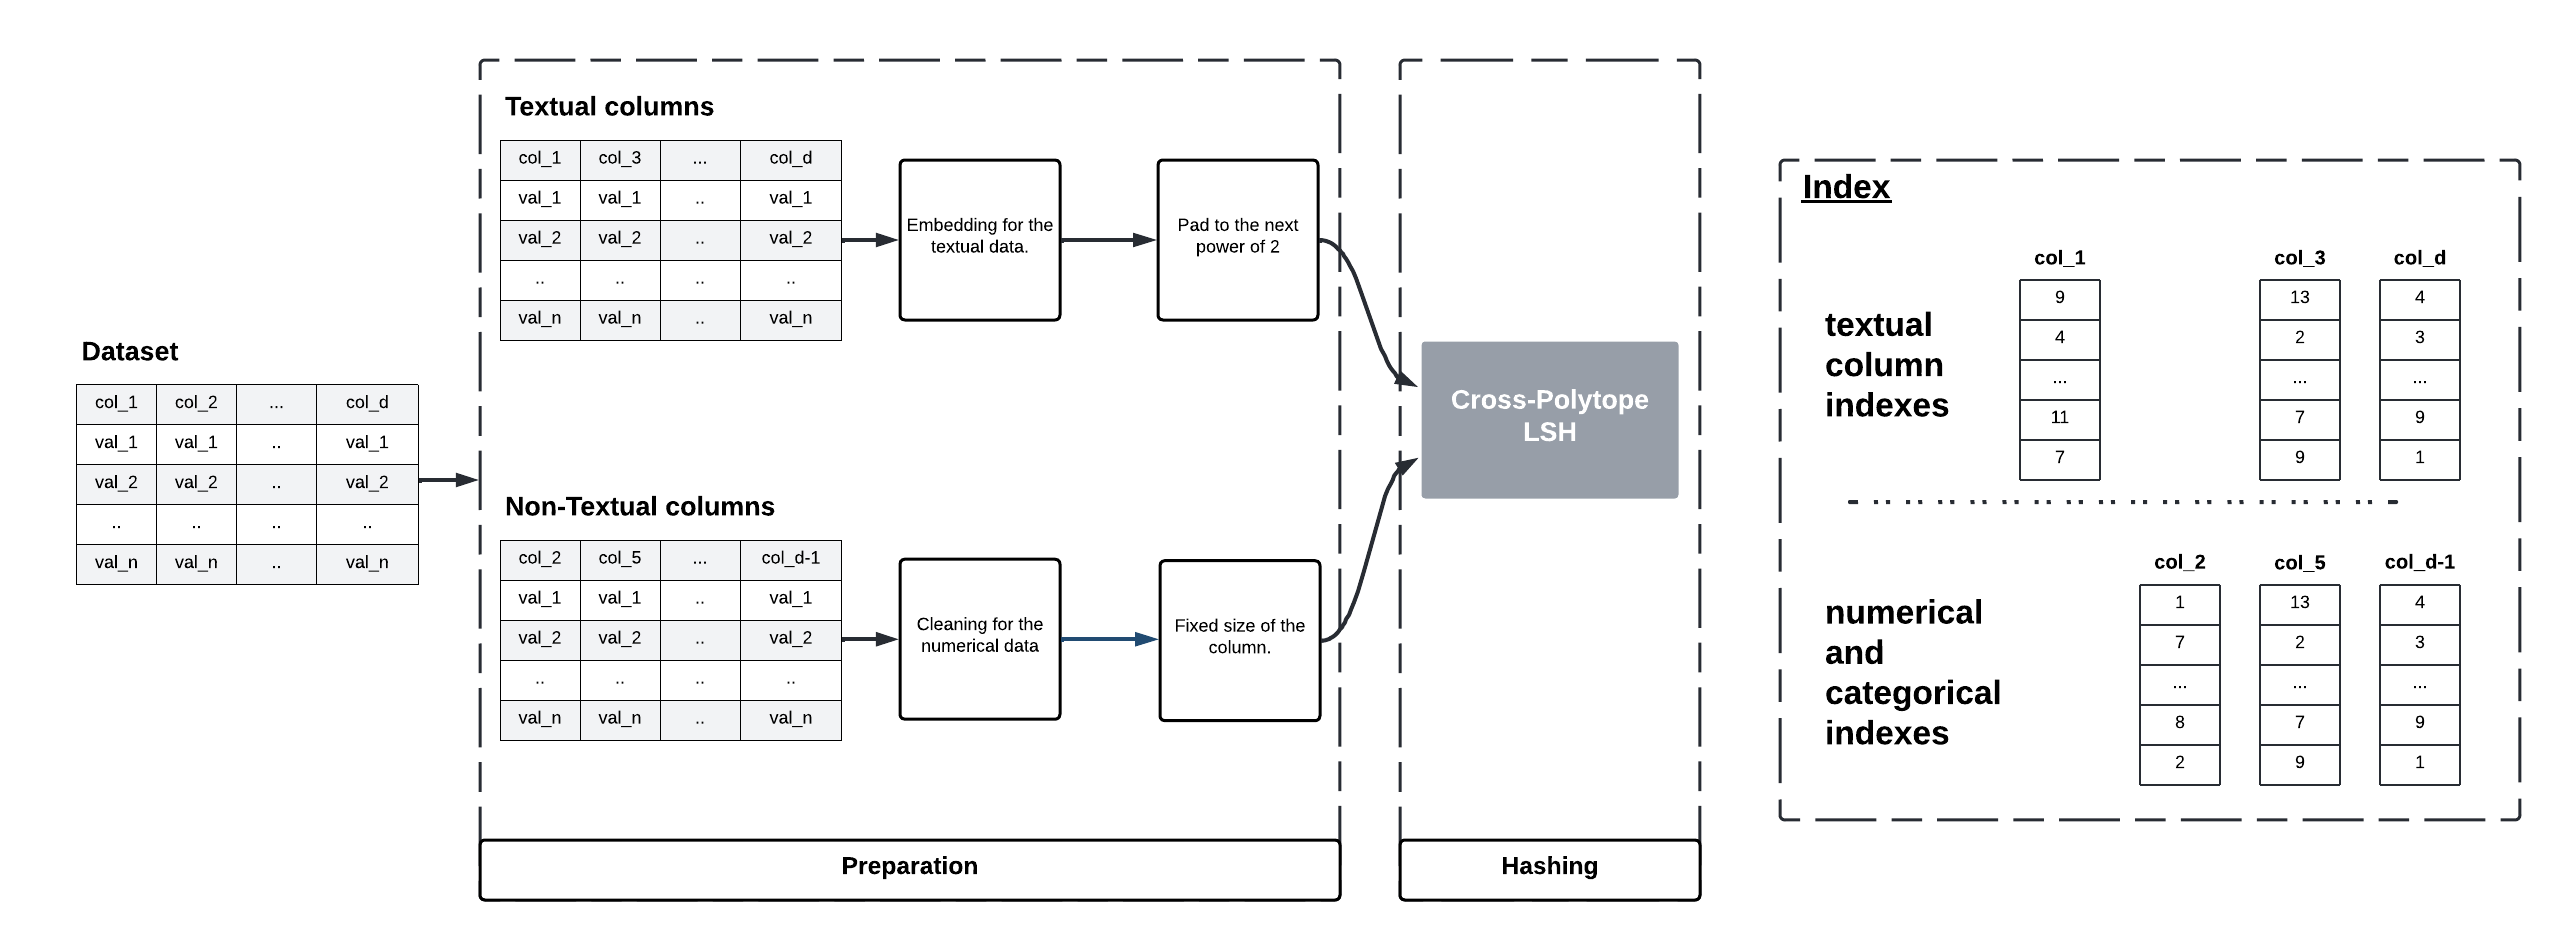
\includegraphics[width=\textwidth]{conception/indexing-whitebg.png}
    \caption{Indexation process illustration}
    \label{fig:indexation_process}
\end{figure}

\subsection{Storing index}
The indexes computed in the previous step need to be stored in order to be used
lately in similarity detection. A key is assigned to every dataset in Talend
Data Inventory, this key is used to store the indexes corresponding to each
dataset. The indexes are stored in a dedicated database which contains the
following attributes:

\begin{itemize}
    \item \textbf{dataset\_id}: Integer. The ID of the corresponding dataset.
    \item \textbf{column\_name}: String. The name of the index column.
    \item \textbf{column\_type}: String. The type of the index column.
    \item \textbf{signature}: Bytes. The encoding of the index.
\end{itemize}


\section{Similarity Detection}
This second part of our solution is meant to proceed for the similarity
detection between two dataset indexes. As described previously, we scale the
similarity detection between dataset to the similarity detection between their
columns, and from the column similarities we can give a score representing the
dataset similarities. 

The process of detecting similarities between columns is
done by the following steps:

\begin{itemize}
    \item Use two groups of bucket, the first one for the textual columns and
    the second for the non-textual column.
    \item Assign each column to a number of buckets depending on its
     calculated index and its type.
    \item Measure the collision rate between the columns that share at least one
    bucket to give their similarity measure (a score between 0 and 1).
\end{itemize}

The similarity measure given by this method is inversely related to the angular
distance, meaning that a score close to 1 represents a high similarity, and a
score close to 0 represents a low similarity.


\section{Implementation}
\label{sect:concep_implementation}
To implement the solution explained in the two previous sections, five different
components have been used:

\begin{itemize}
    \item \textbf{Preprocessing}: It consists of the classes responsible for the
    preprocessing phase, its main class is $DataPreprocessing$ that assures the
    different types of preprocessing (normalization, sampling, embedding..) with
    the use of two other classes, $Embedder$ and $EmbeddingModel$ used to embed
    the textual columns of a dataset.
    \item \textbf{Hashing}: It is the component that assures the indexation
    process, two classes have been used to compute the indexes:
    $CrossPolytope$ and $MultiProbeCrossPolytope$, while the class $Index$ is
    used to represent the index computed for a dataset, 
    \item \textbf{Storing}: It consists of one class that manages the storing
    of the computed indexes
    \item \textbf{Query}: This component gives the features used to detect the
    similarities between indexes through the class $LSHQuery$, and to manage
    their results through the class $QueryResult$
    \item \textbf{Plotting}: With this component, the results given by
    $QueryResult$ are represented graphically with two types of graphs.
\end{itemize}

The figure \ref{fig:class_diagram} represents the class diagram with its
different components as explained in the previous paragraph.

\begin{figure}[h]
    \centering
    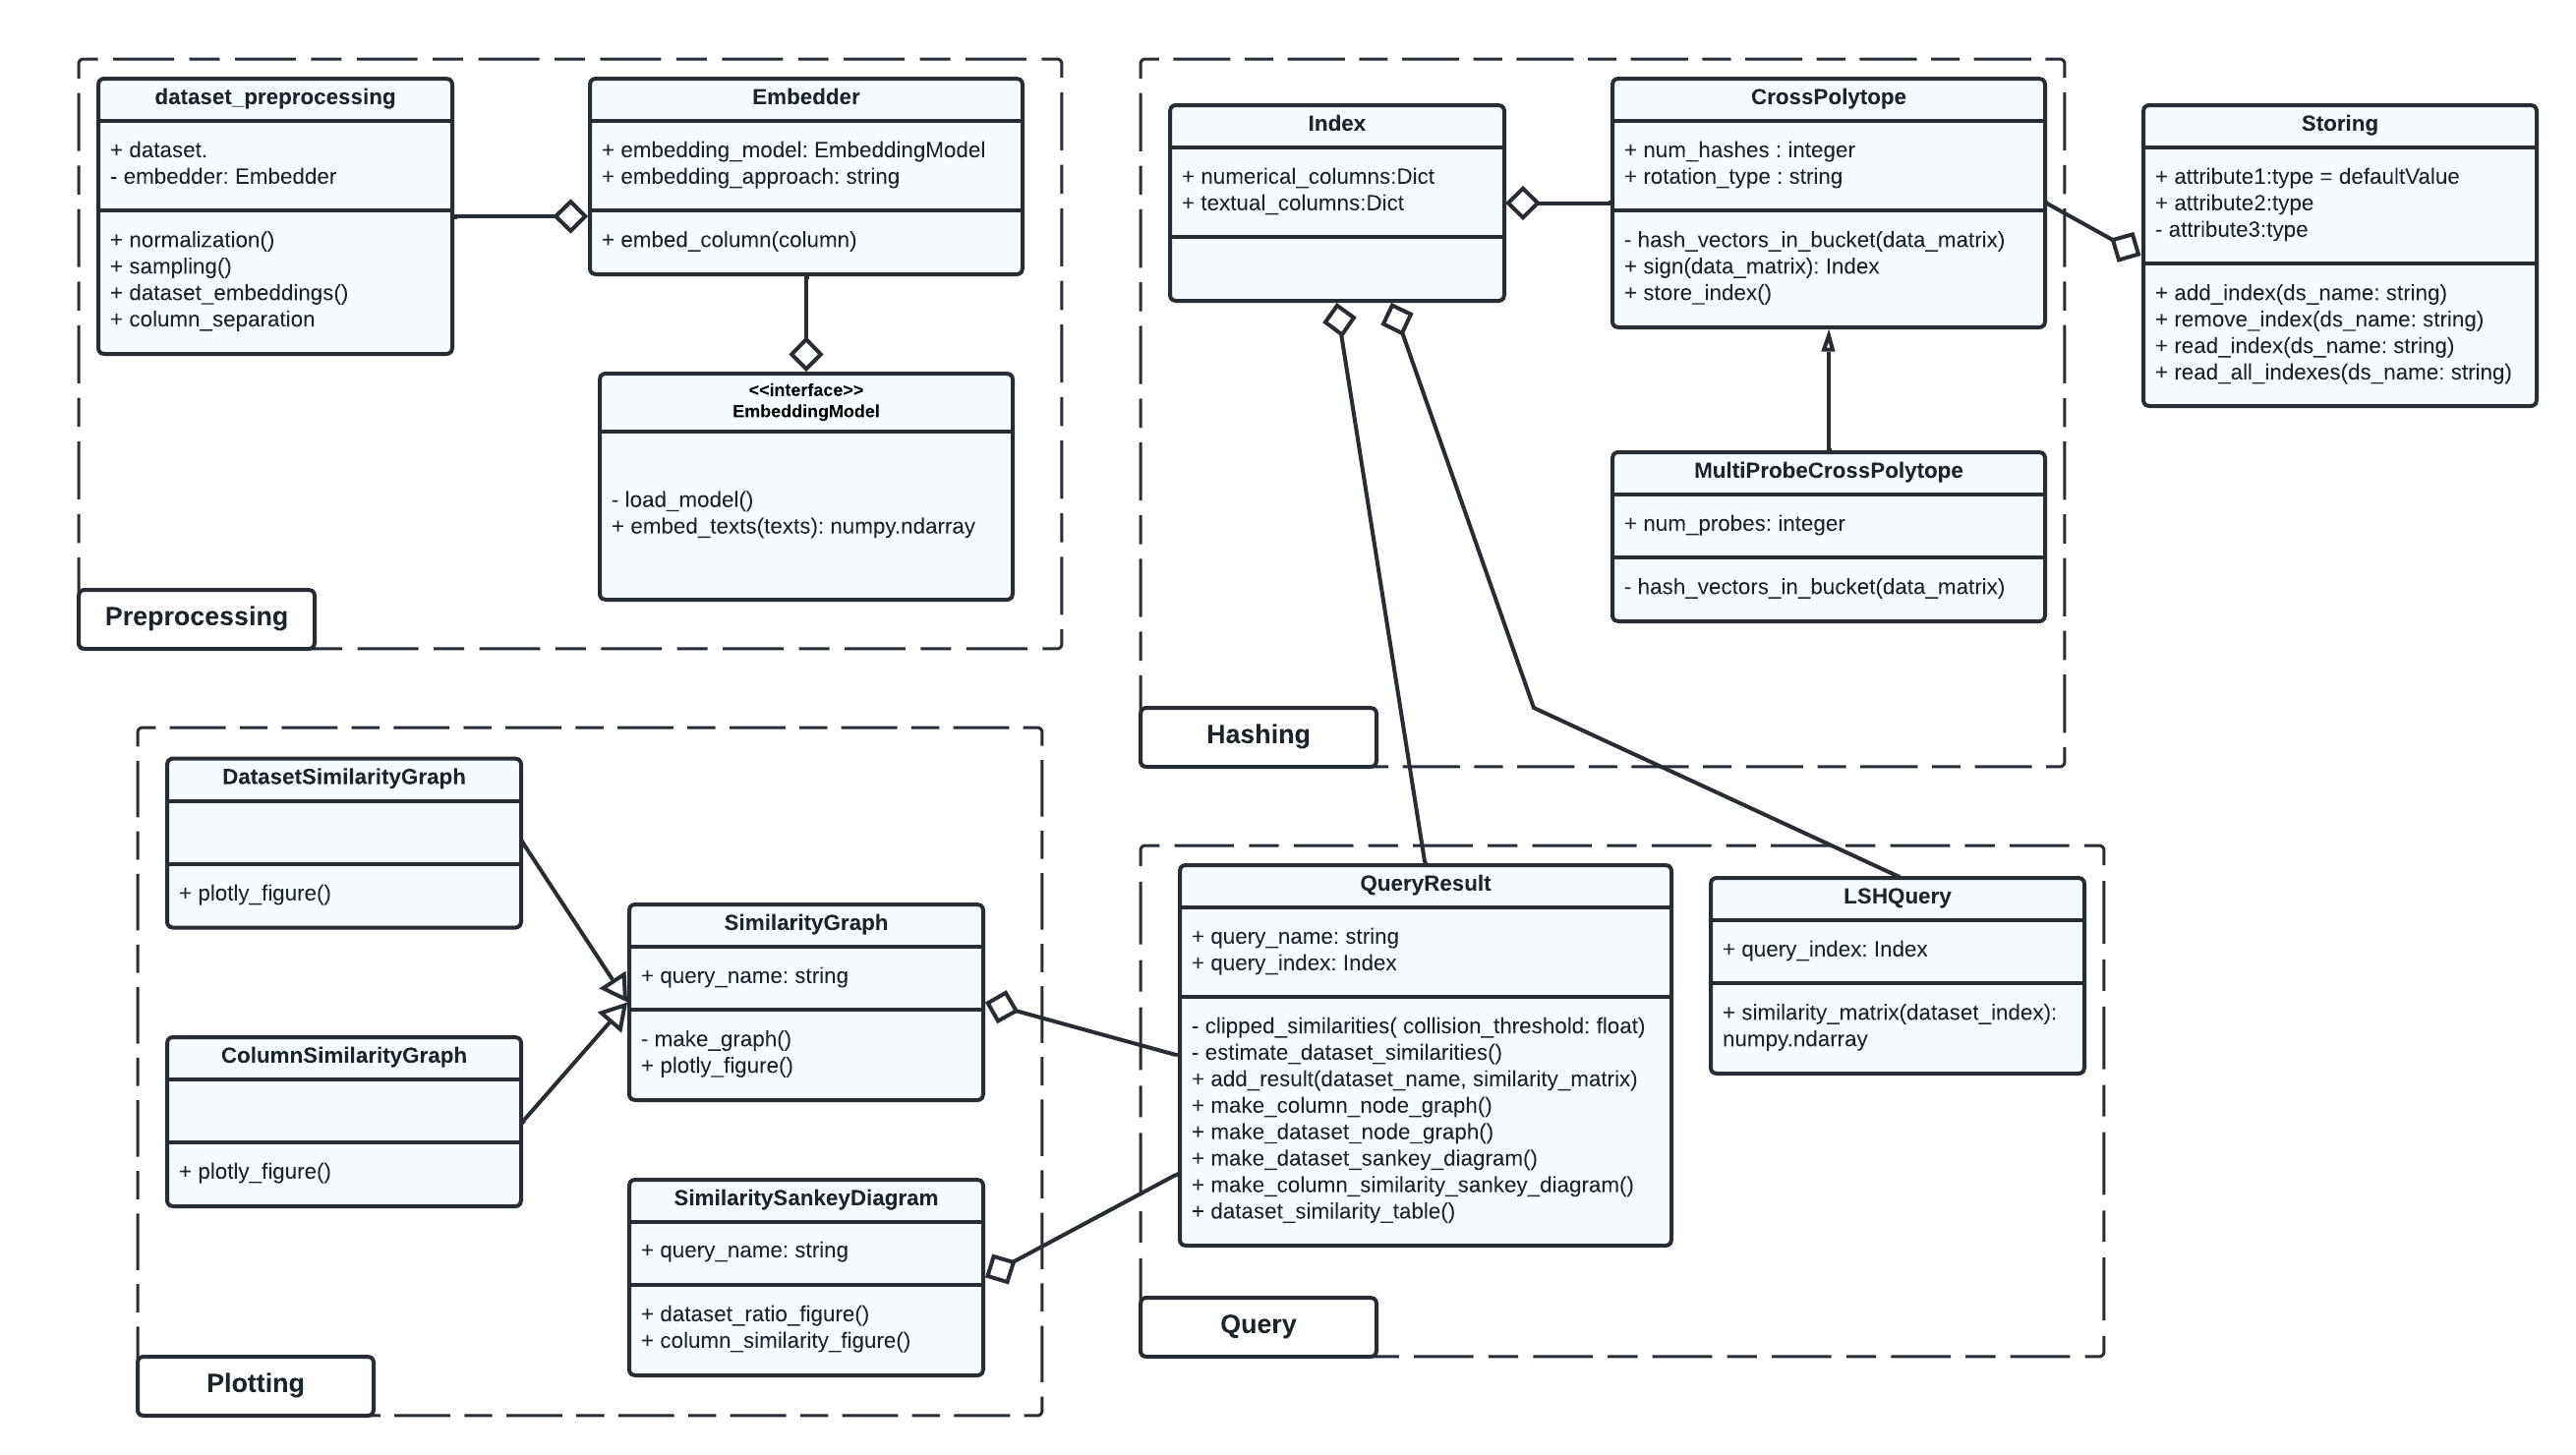
\includegraphics[width=\textwidth]{conception/class-diagram.png}
    \caption{Class Diagram}
    \label{fig:class_diagram}
\end{figure}
\chapter{Realization}
In order to implement the proposed solution, we have proposed a proof of concept
which is a web application built with streamlit that demonstrates the different
features that can be offered.

The use case that we consider in this proof of concept has the following specifications:
\begin{itemize}
    \item The user can select a dataset to be added and indexed.
    \item The user can have the previously indexed datasets.
    \item The user can select a dataset, that we call query dataset, and measure
    its similarities with the other ones.
    \item The computed similarities are presented in two sections:
    \begin{enumerate}
        \item Dataset similarity representation: It orders the dataset by their
        similarity scores with the query datasets.
        \item Column similarity representation: It shows the details of the
        column similarities between the query dataset and a dataset that the
        user selects.
    \end{enumerate}
\end{itemize}


\section{Technologies and tools used}
In order to implement the proposed solution, we have opted for the following
technologies, tools and frameworks:
\subsection{Python}
Python is a structured, open source, multi-paradigm, multi-platform programming
language that runs on all major operating systems and computing platforms. By
offering high-level tools and an easy-to-use syntax, it greatly optimizes the
productivity of programmers and has become a leading language in exploratory
data analysis and software development.

Python have been chosen for implementing this project for the following reasons:
\begin{itemize}
    \item It provides a set of libraries, in the machine learning domain, which
    simplifies the development of our project.
    \item Python manages its resources (memory, file descriptors) without the
    intervention of the programmer, by a reference counting mechanism.
    \item The Lab team of Talend has already used Python in most of their
    projects, this makes it easier to understand, collaborate, scale and
    integrate our solution in the future.
\end{itemize}

We follow up by presenting some of the used libraries during this projet:

\begin{enumerate}
    \item \textbf{Numpy}:
A library used to manipulate matrices, multidimensional arrays, vectors and
polynomials, it has a large number of mathematical functions that can be applied
directly to the structures mentioned above. In this project we have used numpy
to process matrices and arrays.
    
    \item \textbf{Jax}:
Following its definition in its official repository \citep{jax_2022}, Google JAX
is a machine learning framework for transforming numerical functions, the goal
of using this framework is to take advantage from its version of Numpy that
provides us with the possibility of doing the different calculations on GPU. It
shows up that this choice is accurate if we take in consideration the number of
matrix multiplication that we have to do in Cross-Polytope.

    \item \textbf{Pandas}:
Pandas is a python library that allows to easily manipulate data in form of data
tables that we call DataFrame with column and row labels. It provides us with
some interesting easily used features to read, analyze and complete some
preprocessing operations.

    \item \textbf{IGraph}:
It is a library allowing to define and manipulate graphs, it is written in C
programming language and can be used with Python or R. We use it in our solution
to define the graphs representing the results of similarities between columns
and between datasets

    \item \textbf{Plotly}:
Plotly is a complete library for creating static, animated and interactive
visualizations in Python. It is used in our solution to represent the graphs
defined with IGraph with an interactive figures in the streamlit application.

    \item \textbf{Transformers}:
We use the Transformers library which is a state of the art pre-trained model
library for natural language processing (NLP). The library currently contains
pre-trained model weights, user scripts and conversion utilities: Bert,
Roberta...

\end{enumerate}


\subsection{Streamlit}
It is an open source framework in Python language dedicated for data scientist
and machine learning engineers to create complete web applications in a short
time as it provides a set of components that we need to have an interactive
layout. It also provides a compatibility with different Python libraries which
make it easier for building demonstrations that are not exclusive to data
scientists.

Stramlit has also a cloud platform that gives its users the possiblity to
deploy, manage and share their apps.

\subsection{TensorFlow Hub}
It is a repository of trained machine learning models ready for downloading,
fine-tuning or reusing in different projects, with the possiblity to be deployed
everywhere.

We used this library to test different embedding models and choose the most
suitable one in order to get a representation for the textual columns.
\chapter{Experiments and results}
\label{chap:exp_and_tests}
\section{Test and Experiments}
In this section, the focus is on finding the combination of hyper-parameters and
embedding approach leading to the best similarity estimation. To do this we
do our experiments under two metrics.
\begin{itemize}
    \item \textbf{Embedding approach metric}: It consists of applying the
          different embedding approaches proposed in (mention the section when
          it's done) to get the textual column representations of each dataset
          couple, and then measuring the similarities between these
          representations to compare them with the ground truth labels
          \ref{parag:labelled_ds}. The similarities are measured with the
          theoretical collision probability that we estimate by cross-polytope
          LSH:
          \begin{equation}
              \label{equ:cp_exact_measure}
              P(h(x) = h(y)) = \exp{- \frac{\pi ^2}{4 - \pi ^2}. \ln{d}}
          \end{equation}.
    \item \textbf{Cross-Polytope hyper-parameters:} It consists of estimating
          the similarities with cross-polytope using different values for the
          two parameters: number of hashing functions to use, and the number of
          probes, and computing the error of this estimation to the theoretical
          collision probability (\ref{equ:cp_exact_measure}).
\end{itemize}

\paragraph{The set of labelled similarities}:
\label{parag:labelled_ds}
It is a dataset containing
different sets of datasets associated with lists of columns that can be matched.
It is a human labelling done in a previous project at Talend. This labelled
datasets are organized as the following example:
\begin{center}
    \begin{tabular}{|c | c | c | c|}
        \hline
        \textbf{dataset 1} & \textbf{dataset 2} & \textbf{column dataset 1} &
        \textbf{column dataset 2}
        \\
        \hline
        students           & clients            & Student Name              &
        client name                                                           \\
        \hline
        students           & clients            & inscription data          &
        join date                                                             \\
        \hline
        students           & clients            & Gender                    &
        gender                                                                \\
        \hline
        books              & publications       & release data              &
        publication date                                                      \\
        \hline
        $\cdot$            & $\cdot$            & $\cdot$                   &
        $\cdot$                                                               \\
        \hline
        books              & publications       & title                     &
        title                                                                 \\
        \hline
    \end{tabular}
\end{center}

To each couple of labelled dataset with their respective similar columns, a
label matrix is associated to represent their similarities with the following
process:

\begin{figure}[h]
    \centering
    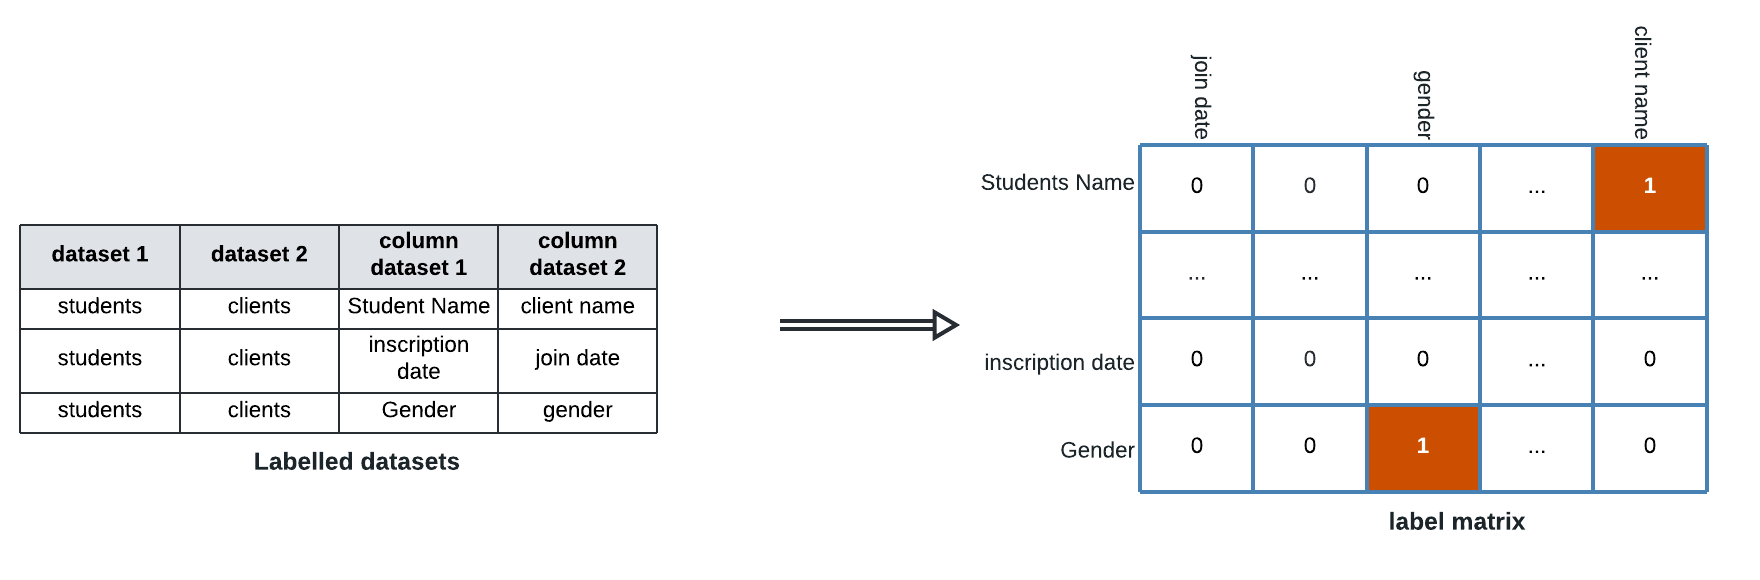
\includegraphics[width=\textwidth]{tests/labelled_entry.png}
    \caption{Label matrix generation from the labelled column similarities}
    \label{fig:label_matrix}
\end{figure}

\subfile{tests/01-embedding_metric.tex}

\subfile{tests/02-index_hp.tex}
\chapter*{Conclusion}
\addcontentsline{toc}{chapter}{Conclusion}

This internship period has been full and rich in terms of acquiring new
experiences and skills. It was an experience that not only allowed me to learn
more about the field of machine learning, but it was also an opportunity to
develop on the organizational side, in terms of work methodology, quality of
exchanges, requirements on deliverables and the importance of software
engineering itself. 


Through this report, I have exposed the work done in the project of my graduation
internship which consisted in doing a state of the art and an implementation to
address the need of having a tool able to detect the similarities between
dataset based on their content with Cross-Polytope which is a \acrfull{lsh}
method.

I started this report with a definition on the \acrfull{nns} problem, how need
it is to scale it to \acrfull{ann} and I exposed the metrics that it can use to
measure the similarities or dissimilarities between data points. I continued by
presenting \acrshort{lsh} family of methods as one of the methods that tackle
\acrshort{nns}, I explained its global approach and finally presented their
different methods related to each one of the previously mentioned metrics.

My solution starts by initiating a set of preprocessing over the dataset, it
first needs to get its columns separated into textual and non-textual column,
embed the textual ones and get a sample from the second one. This solution is
based on indexing the columns after preprocessing with Cross-Polytope LSH, a
method that gives an estimation related to the angular distance. And to get the
similarity measures with this solution, we need to get the buckets of each
column with its indexes, and then compute the similarity between the indexes that share at least one bucket.


\section*{Perspective}
Despite the good results shown by this solution, there is still work to be done
before it goes into production. This work will be mainly to see how to integrate
it as a feature in Talend Data Inventory, and to get the first feedbacks from
the users taking in consideration that they can have datasets in different forms
and with so many types, something that couldn't be guaranteed with the benchmark
we used for the tests.

\printnoidxglossary[nonumberlist]
\clearpage

\bibliographystyle{apalike}
\bibliography{database}

\end{document}
